\documentclass{article}

\usepackage{corl_2017}

\usepackage{natbib}
\usepackage[english]{babel}
\usepackage[utf8]{inputenc}
\usepackage{amsmath}
\usepackage{graphicx}
\usepackage[colorinlistoftodos]{todonotes}
\usepackage{booktabs}

\usepackage{tikz}
\usetikzlibrary{math,fpu,calc,fit,mindmap,backgrounds,positioning}

\usepackage{xspace}
\newcommand{\eg}{e.g.\xspace}
\newcommand{\etal}{et al.\xspace}
\newcommand{\ie}{i.e.\xspace}
\newcommand{\etc}{etc.\xspace}
\newcommand{\vs}{\textit{vs.}\xspace}

\graphicspath{{figs/}}

\title{PInSoRo: A Dataset for Deep-learning of Human-Robot Social Interactions}


\author{Séverin Lemaignan, Charlotte Edmunds, Tony Belpaeme}

\date{\today}

\begin{document}
\maketitle

\begin{abstract}

%% Original abstract -- kept for future reference
%Over the last decades, efforts around the world have sought to improve
%human-robot interactions, more recently with a focus on longer-term
%interactions. If worthy, these efforts are often incremental and many
%problems remain. In the light of the recent and rapid progress of machine
%learning, we propose here to shift the paradigm: instead of more and more
%complex symbolic cognitive modeling of the interactions between humans and
%robots, we argue that natural and sustainable human-robot interaction could
%instead be directly learned from actual human-human interactions. This paper
%outlines the main challenges ahead, and proposes a first concrete step
%toward the operationalization of this novel paradigm: the creation of a
%large dataset of human-robot social interactions, suitable for machine
%learning.

Child-robot interactions are increasingly being explored in domains which
require longer-term application, such as healthcare and education. In order
for a robot to behave in an appropriate manner over longer timescales, its
behaviours should be coterminous with that of the interacting children.
Generating such sustained and engaging social behaviours is an on-going research
challenge, and we argue here that the recent progress of deep machine learning
opens new perspectives that the Human-Robot Interaction (HRI) community
should embrace.

As an initial step in that direction, we introduce a novel
open dataset of children social interactions, designed with
deep-learning applications in mind. Our acquisition methodology relies on
engaging and purposefully underspecified \emph{free play} situations. By doing
so, we capture a rich set of behavioural patterns occurring in natural
social interactions. Learning to recognise (and generate) automatically such
behaviours is one of the ambitious foreseen outcome that this dataset enables.


\end{abstract}

\section{Machine Learning: the Next Horizon for Social Robots?}

While the family of recurrent neural networks (RNN) have repeatedly made the
headlines over the last few years with impressive results, notably in image
classification, image labelling and automatic translation, they have been so far 
largely ignored by  many other fields as they are perceived to require very
large datasets (hundreds of thousands to millions of observations) to actually
build up useful capabilities. Even though neural networks have demonstrated
compelling results in open-ended, under-specified tasks like image labelling, they
did not stand out as attractive approaches to problems involving high dimensions
with relatively small datasets available -- like human-robot social
interactions.

Besides, if one considers ``social interactions'' to also entail joint
behavioural dynamics, and therefore, some sort of temporal modeling, neural
networks look even less enticing as time is notably absent from most of the
tasks which neural networks have been successful at.

In 2015, the Google DeepMind team demonstrated how a convolutional
recurrent neural network could learn to play the game Break-Out (amongst
48 other Atari games) by only \emph{looking} at the gaming console
screen~\cite{mnih2015human}. This result represents a major milestone: they show
that a relatively small sample size (about 500 games) is sufficient for an 
artificial agent to not only learn how to play (which requires an implicit model 
of time to adequately move the Break-Out paddle), but to also create gaming 
strategies that \emph{look like} they would necessitate planning (the system first
breaks bricks on one side to eventually get the ball to break-out and reach the area
\emph{above} the remaining bricks, therefore ensuring rapid progress in the
game).

More recently, Ogata's team~\cite{yang2017repeatable} has demonstrated how an
adequately configured RNN is able to learn a complex robotic task (folding soft
objects like towels using a dual-arm mobile manipulator) from only \emph{35}
demonstrations, one demonstration being a $\approx$ 70 seconds-long teleoperated
sequence. The network inputs are the raw video stream from the head camera and the
12 DoF of the two arms and the total training dataset comprises of about 28000
steps of data. Successfully folding towels entails an explicit sequencing of
actions (therefore implicit temporal modeling). The fact that such a complex
process can be successfully learned from a very small dataset certainly opens
many prospects.

Indeed, we argue that the complexity of mechanisms that such neural networks
have been able to uncover and model should invite our community to question its
applicability to human-robot interactions in general, and sustained, natural
child-robot interactions in particular.
However, the current lack of an appropriate HRI dataset suitable for the training of
neural networks hinders this investigation. We present hereafter such a dataset,
and detail our acquisition methodology.

\subsection*{Machine Learning and Social Behaviours}

The use of interaction datasets to teach robots how to socially behave has been
previously explored, and can be considered as the extension of the traditional
learning from demonstration (LfD) paradigms to social interactions (for
instance~\cite{nehaniv2007imitation,mohammad2015interaction}). Previous examples
have generally focused on low-level recognition or generation of short,
self-standing behaviours, including social gestures~\cite{nagai2005learning} and
gazing behaviours~\cite{calinon2006teaching}.

Based on a human-human interaction dataset, Liu \etal~\cite{liu2014how} have
investigated machine learning approaches to learn longer interaction sequences.
Using unsupervised learning, they train a robot to act as a shop-keeper,
generating both speech and socially acceptable motions. Their approach remains
task-specific, and while they report only limited success, they emphasise the
``life-likeness'' of the generated behaviours.

Kim \etal~\cite{kim2015pororobot} highlight that applying deep learning to
visual scene information in an HRI scenario was successful, but that
generating behaviours for the robot to be able to act in a dynamic and uncertain
environment remains a challenge.
They rely on unsupervised learning, with a
training stage consisting in clustering behavioural states (a state consist in
\emph{behavioural elements} (joint states of the two interacting agents,
associated to the current speech elements, as well as the current joint
\emph{spatial formation}), followed by the \todo[inline]{finish that}.

These examples show the burgeoning interest of our community for the automatic
learning of social interactions, but also highlight the lack of structure of
these research efforts, as further illustrated by the lack of large, open
datasets of social interactions, suitable for machine-learning applications.

One interesting dataset is the \emph{Multimodal Dyadic Behavior
Dataset} (\emph{MMDB},~\cite{rehg2013decoding}). It comprises of 160 sessions of
3 to 5 minute child-adult interactions. During these interactions, the
experimenter plays with toddlers (1.5 to 2.5 years old) in semi-structured ways.
The dataset includes video streams of the faces and the room, audio, physiological data
(electrodermal activity) as well as manual annotations of certain behaviours
(like gaze to the examiner, laughter, pointing). The lack of calibration and camera positioning
information in the dataset limits the possibilities of automatically extracting and
labelling key interaction features (like facial expressions or joint gaze). Besides,
this dataset focuses on very young children with in adult-driven interactions,
and as such does not include any episodes of naturally-occurring social
interactions between peers.

\todo[inline]{look at other child-child datasets!}
\todo[inline]{mention research on deep-learning to diagnose autism}

\section{The Plymouth Interacting Social Robots Dataset (PInSoRo)}

\todo[inline]{the dataset is not specific to robotics...PinSoRo is maybe not the
    best name?}

The Plymouth Interacting Social Robots (PInSoRo) Dataset comprises of natural
social interactions arising between children, and recorded with machine learning
applications in mind.

As detailed in section~\ref{availability}, this dataset is open and made freely
available to any interested researcher. It is intended to be used to train
machine-learning algorithms (typically, deep recurrent networks) to both
recognise and generate complex cognitive and social dynamics occurring in the
wild during social interactions.

\subsection{The Freeplay Sandbox}

\begin{figure}
    \centering
    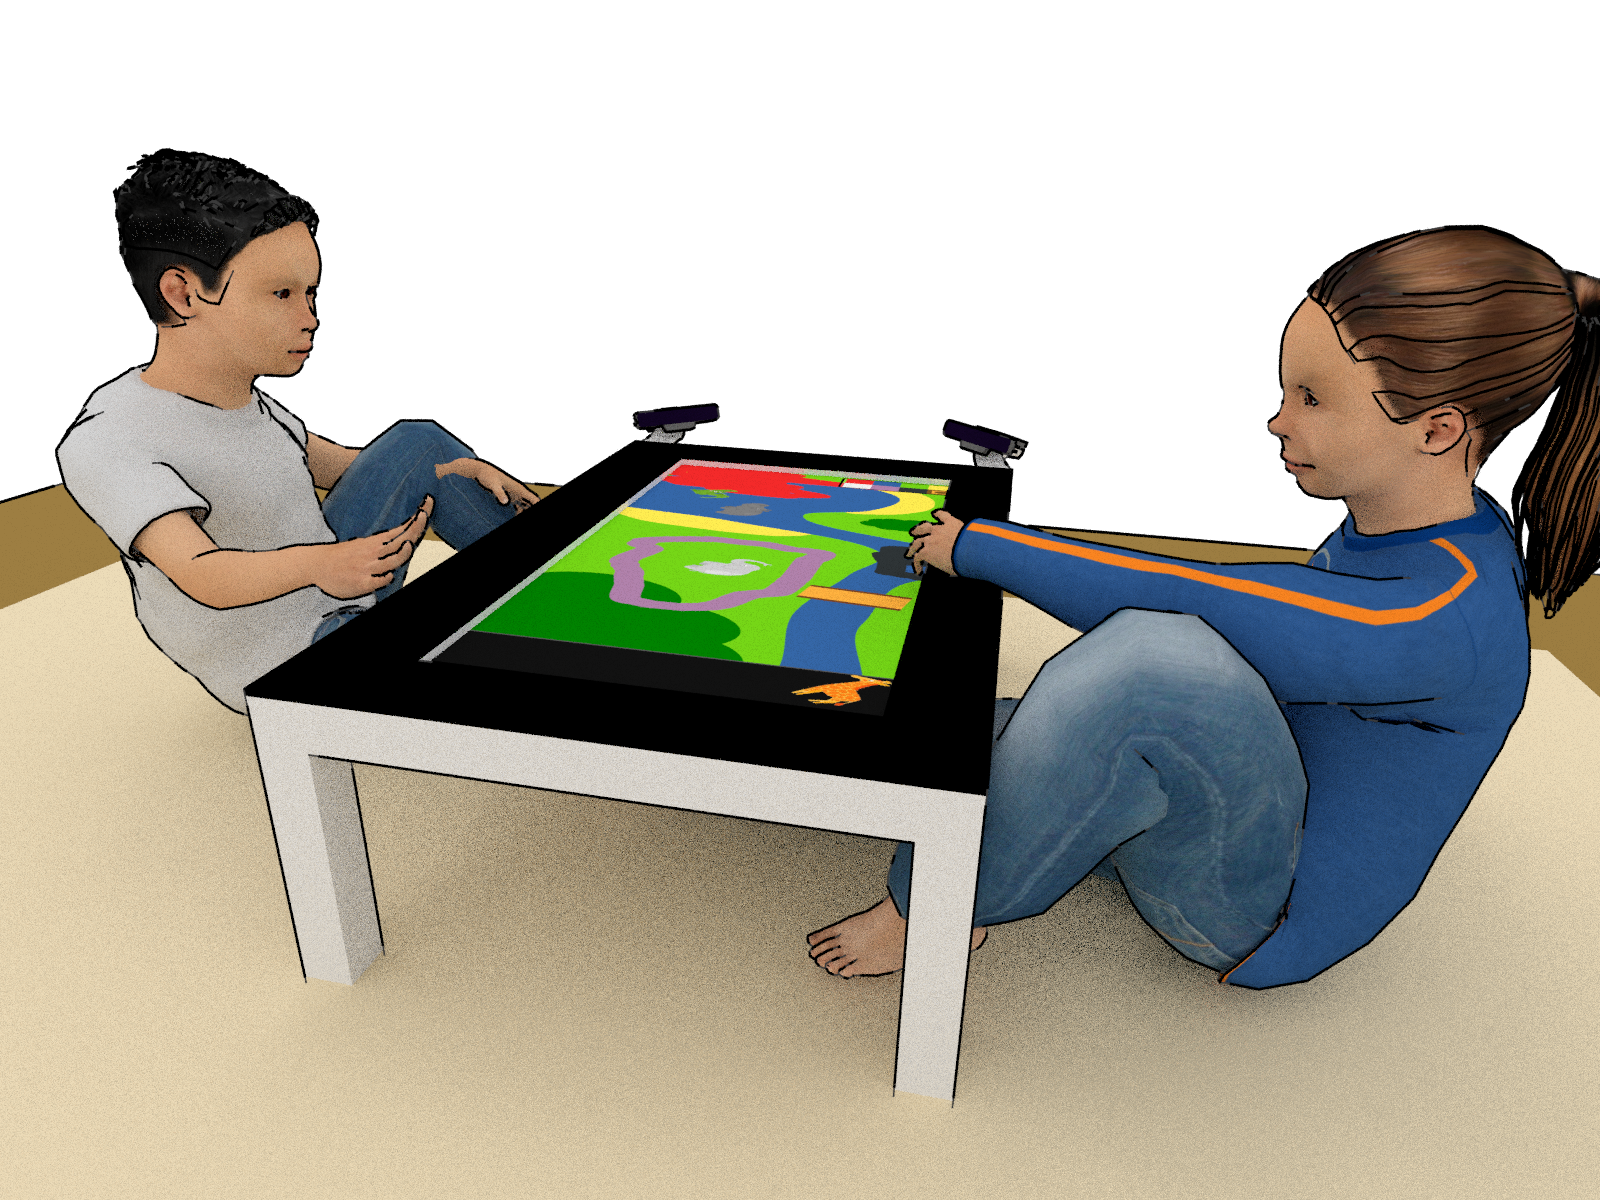
\includegraphics[width=0.4\linewidth]{setup-child-child.png}
    \hspace{1em}
    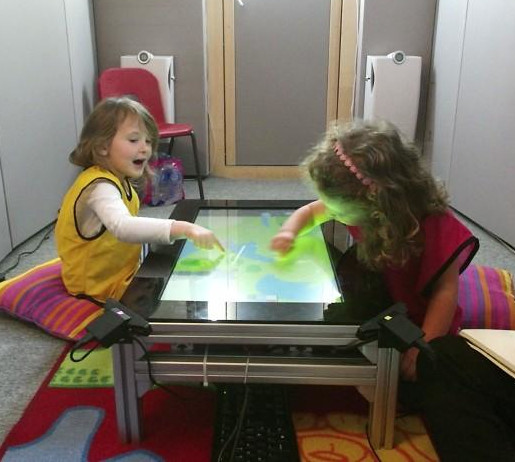
\includegraphics[width=0.4\linewidth]{child-child-env}
    \caption{The free play social interactions sandbox: two children interact in
    Da free-play situation, by drawing and manipulating items on a touchscreen.}
    \label{fig|setup}
\end{figure}

The acquisition of such a dataset requires first the definition of a suitable
task for the participants to perform while they are recorded. The nature of
this task influences in fundamental ways the kind of interactions that might be
observed, and thus, learned. Because they usually target very specific social
or cognitive skills in a tightly controlled manner, traditional socio-cognitive tasks are
usually simple, constrained tasks that do not reflect the complexity and dynamics of
real-world interactions. On the contrary, this dataset aims at capturing a rich set
of naturally-occurring social interactions. As such, a suitable task has to be:

\begin{itemize}
    \item elicit a large range of interaction situations;
    \item foster rich multi-modal interaction: simultaneous speech, gesture, and gaze
        behaviours are to be observed;
    \item fundamentally social, \ie the task would make little sense for an
        agent alone;
    \item foster non-trivial social dynamics, such as implicit turn-taking.
\end{itemize}

We present a new experimental task based on \emph{free play} interactions. Pairs of
children (4-7 years old) are invited to freely draw and interact with items
displayed on an interactive table, telling and acting stories with no explicit
goal set in advance (Fig.~\ref{fig|setup}).

In order to constraint the dataset to a tractable domain, the task is limited to
a dyadic \emph{face-to-face} interaction.  The resulting interaction space is
nevertheless high-dimensional, with two main axis: the game-related actions
(drawing, manipulating items, telling stories) and the social interactions
(monitoring the other's actions, discussing and agreeing on joint actions,
helping behaviours, etc.).

The \emph{freeplay sandbox} follows the sandtray
paradigm~\cite{baxter2012touchscreen}: a large touchscreen (60cm $\times$ 33cm,
multitouch) is used as an interactive surface (\emph{sandtray}). The two children play together
by freely moving interactive items (Fig.~\ref{fig|sandbox}) on the surface. A background image
depicts a generic empty environment, with different symbolic zones (water,
grass, path, bushes...). The players do not have any particular task to
complete, they are simply invited to freely play.
is implemented wit To mitigate the technical challenges presented by free play interactions in
their most unconstrained version (like
high dimensionality and uncertainties), we have developped a \emph{free play
sandbox}, Fig.~\ref{fig|setup}: 


\begin{figure}
    \centering
    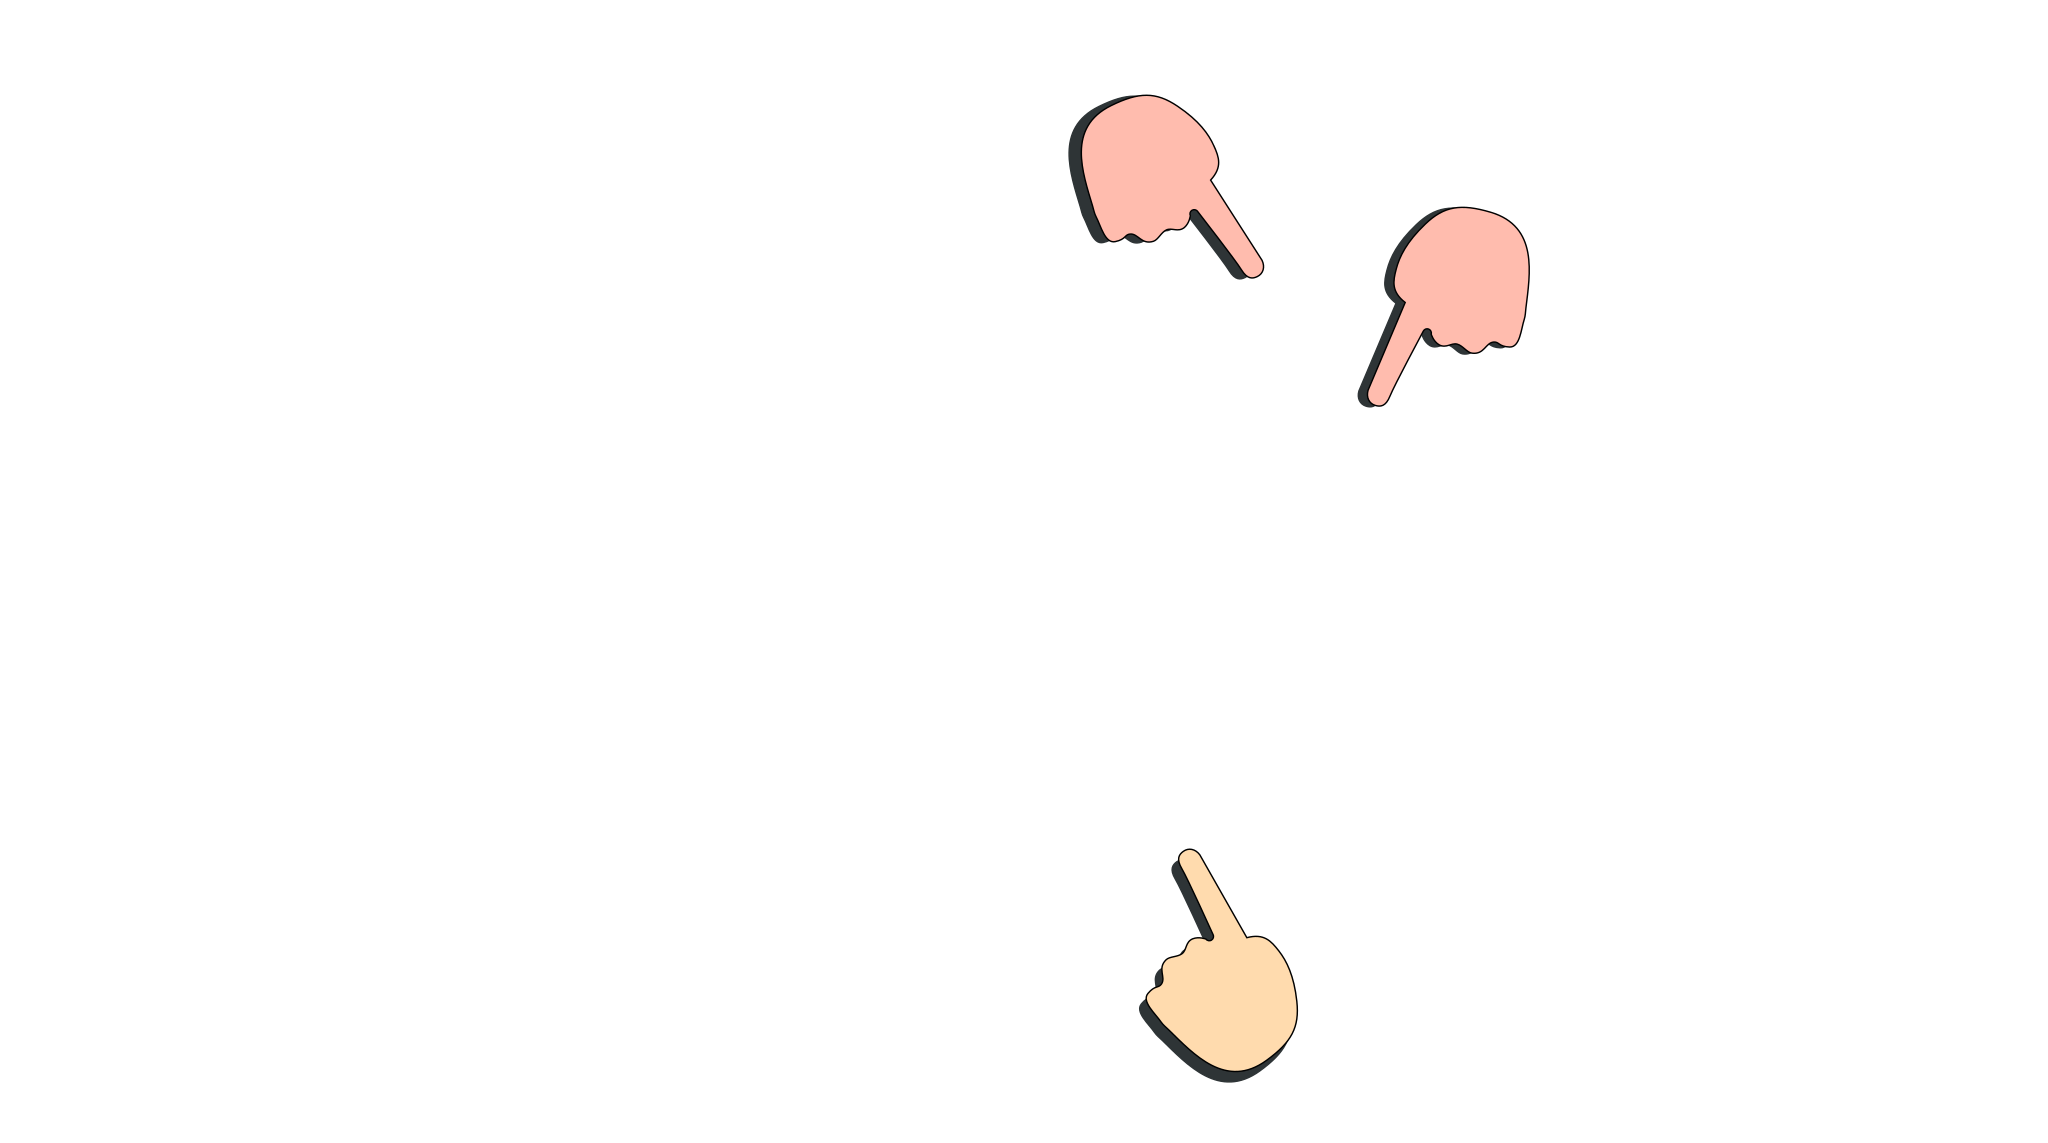
\includegraphics[width=0.9\linewidth]{sandbox}
    \caption{Example of a game situation: the two children `build'
    together a zoo. Items (animals, characters...) can be dragged over the whole
    play area, while the background picture can be painted over by picking a
    colour.}
    \label{fig|sandbox}
\end{figure}




children can engage in open-ended and
non-directive play situations, yet sufficiently
defined to be reproducible; 

\subsubsection{Socio-cognitive Framing}

focus on abstract socio-cognitive facets (robot
perception and manipulation are simplified); well suited for qualitative and
quantitative analysis using metrics like Słowinski’s Individual Motor Signature
(for behavioural alignment), Anderson's~\cite{anderson2004social} coding of children’s free-play
interactions, with-me-ness (for assessment of co-engagment).

carefully framed: as far as possible, they ne-
cessitate only the cognitive capabilities that they ev-
idence (e.g. if they evidence a purely socio-linguistic
mechanism, they will not mandate complex action ca-
pabilities – they may benefit from it, though),

This point is especially important as it allows an
incremental path: a robot should be able to tackle one or
several of these task independently of the others, and a re-
search team may progressively extend their cognitive models
to incorporate more and more of the cognitive capabilities
required by the robot to address all of the tasks.



\subsubsection{Implementation}

The sandbox is implemented using mainly two frameworks: the Qt's \emph{QtQuick} framework
for the graphical interface of the game, and the \emph{Robot Operating System}
(ROS) for the modular implementation of the data processing and behaviour
generation pipelines.

\begin{figure}
    \centering
    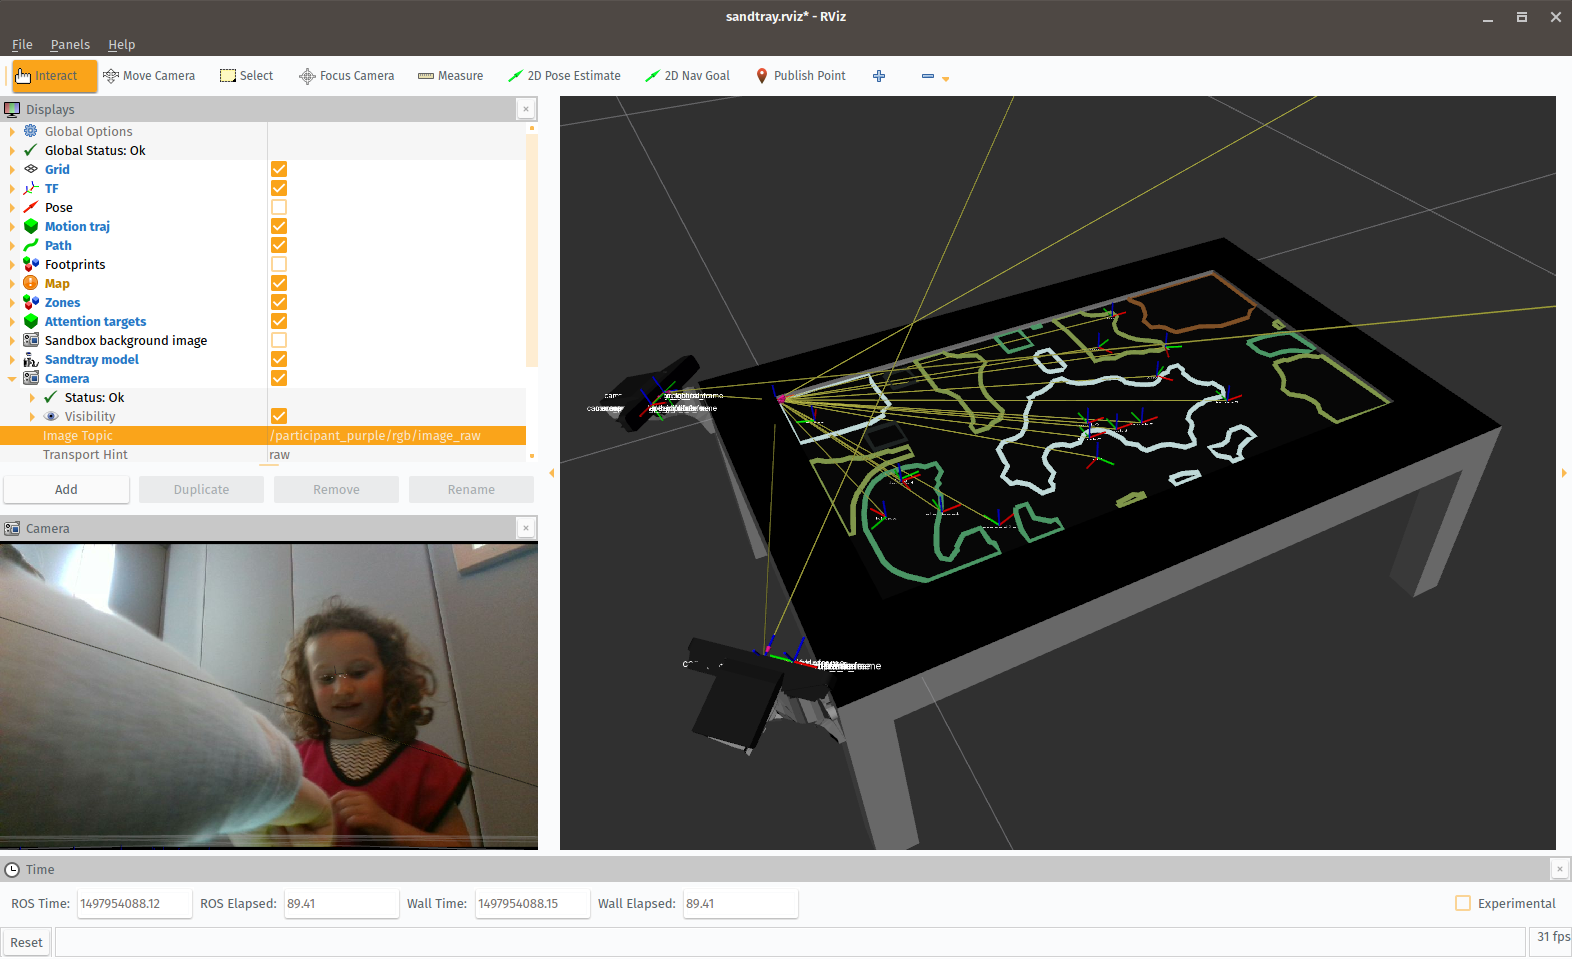
\includegraphics[width=0.9\linewidth]{rviz-sandtray}
    \caption{The freeplay sandbox, viewed at runtime within ROS RViz. The
    current background drawing is published on a regular image
    topic and computer vision is used to segment it into zones (visible in
    the central panel). The poses and bounding boxes of the interactive items
    are published as well, and turned into an occupancy map, used to plan the
    robot's arm motion.}
    \label{fig|rviz}
\end{figure}

\subsection{Dataset Acquisition}

All data has been collected by researchers at the Plymouth University, under a
protocol approved by the university ethics committee. The parents of the
participants explicitly consented to sharing of their child's video and audio
with the research community. The data is labelled with a unique participant code
only and does not contain any identifying information, except the participant's
images. The child's age and gender are also available.

\begin{figure}
    \centering
    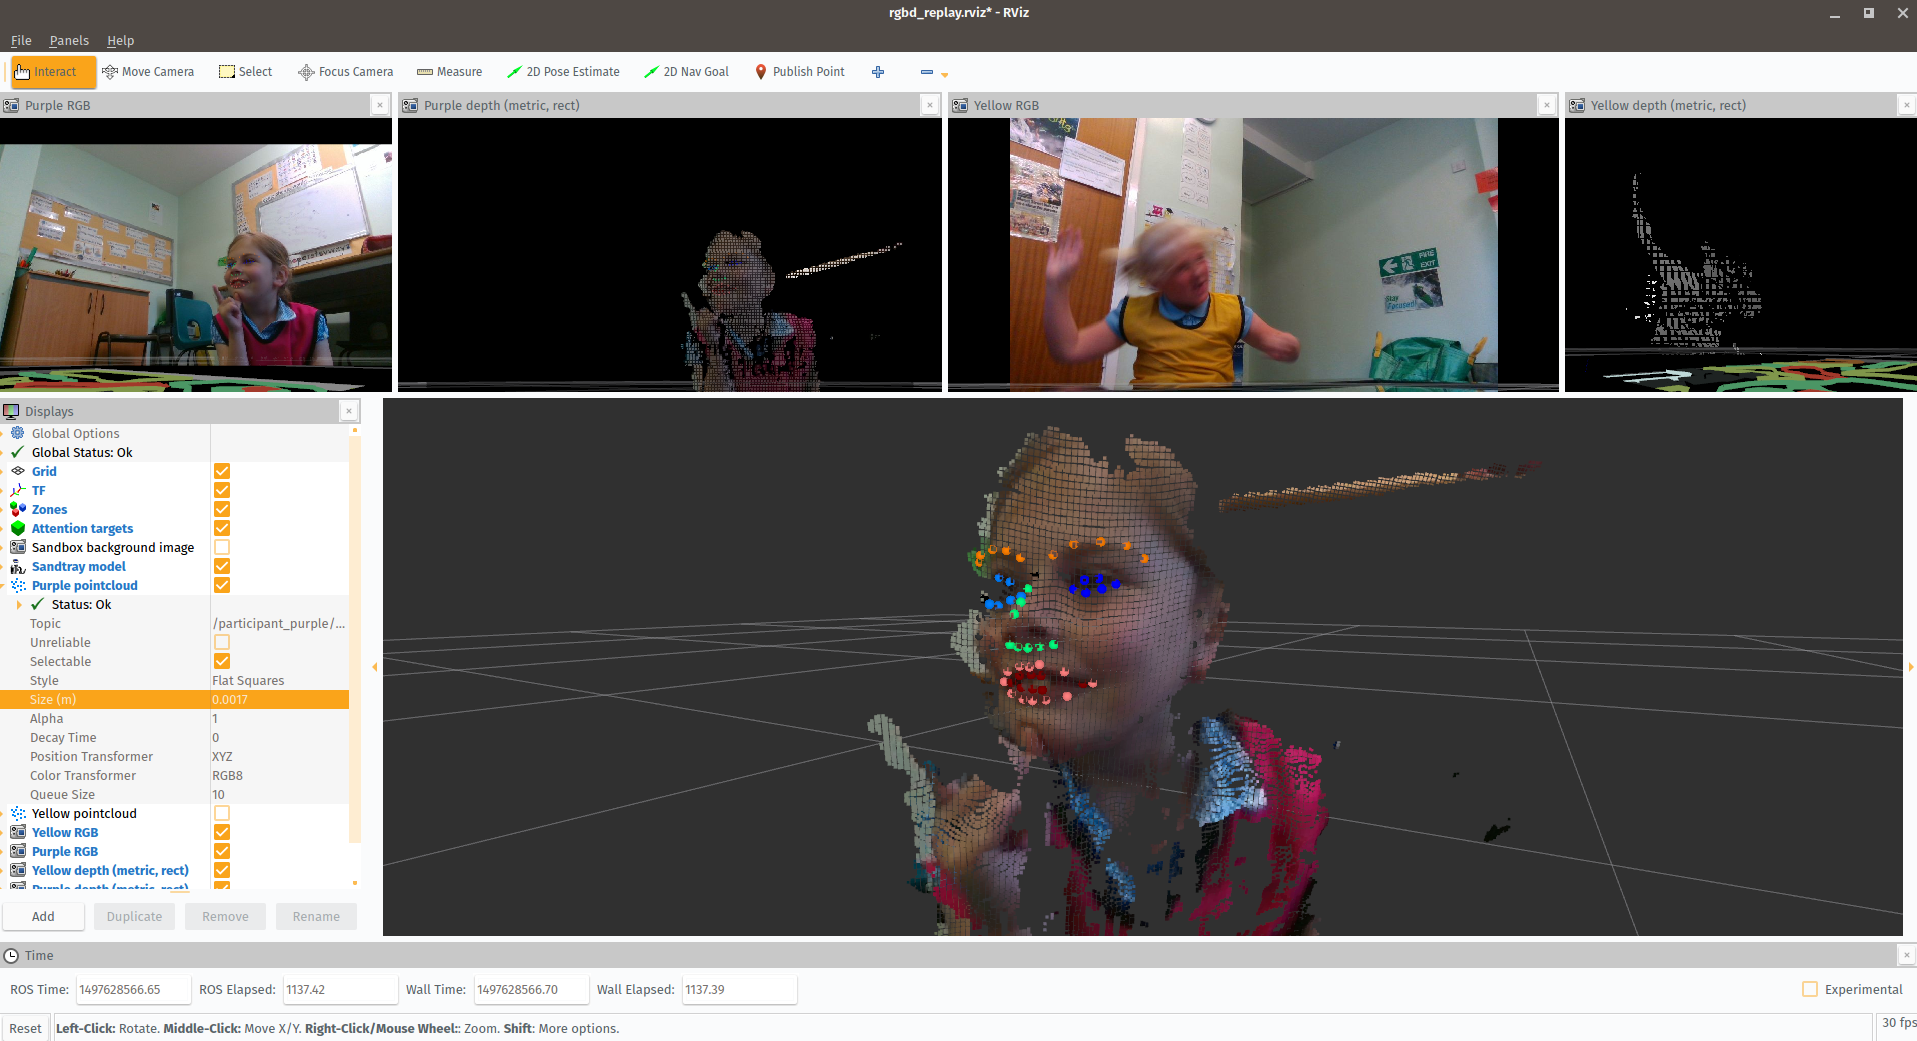
\includegraphics[width=0.9\linewidth]{3d-point-cloud-facial-features}
    \caption{Reconstructed 3D point cloud with 68 facial features high-lighted}
    \label{fig|pointcloud}
\end{figure}

\subsubsection{Conditions}\label{conditions}

\begin{itemize}
\item
  Condition A: one pair of children freely play together on the
  sandtray.
\item
  Condition B: one child play together with the robot, the robot does
  not exhibit any social behaviour.
\end{itemize}

\subsubsection{Demographics}\label{demographics}

\begin{itemize}
\item
  Condition A: 40 pairs of children (ie, 80 children)
\item
  Condition B: 40 children
\end{itemize}

2 age groups, balanced across conditions: 4 y.o. (nursery) and 6 to 7
y.o. (Y1/Y2)

Normally developping children, from local primary schools and nurseries.



\subsubsection{Experimental Setup}\label{experimental-setup}

On large touchscreen, mounted on a horizontal frame (\emph{sandtray});
both children (condition A, Figure 2) or the child and the robot
(condition B, Figure 3) are facing each other.

\begin{figure}[htbp]
    \centering
    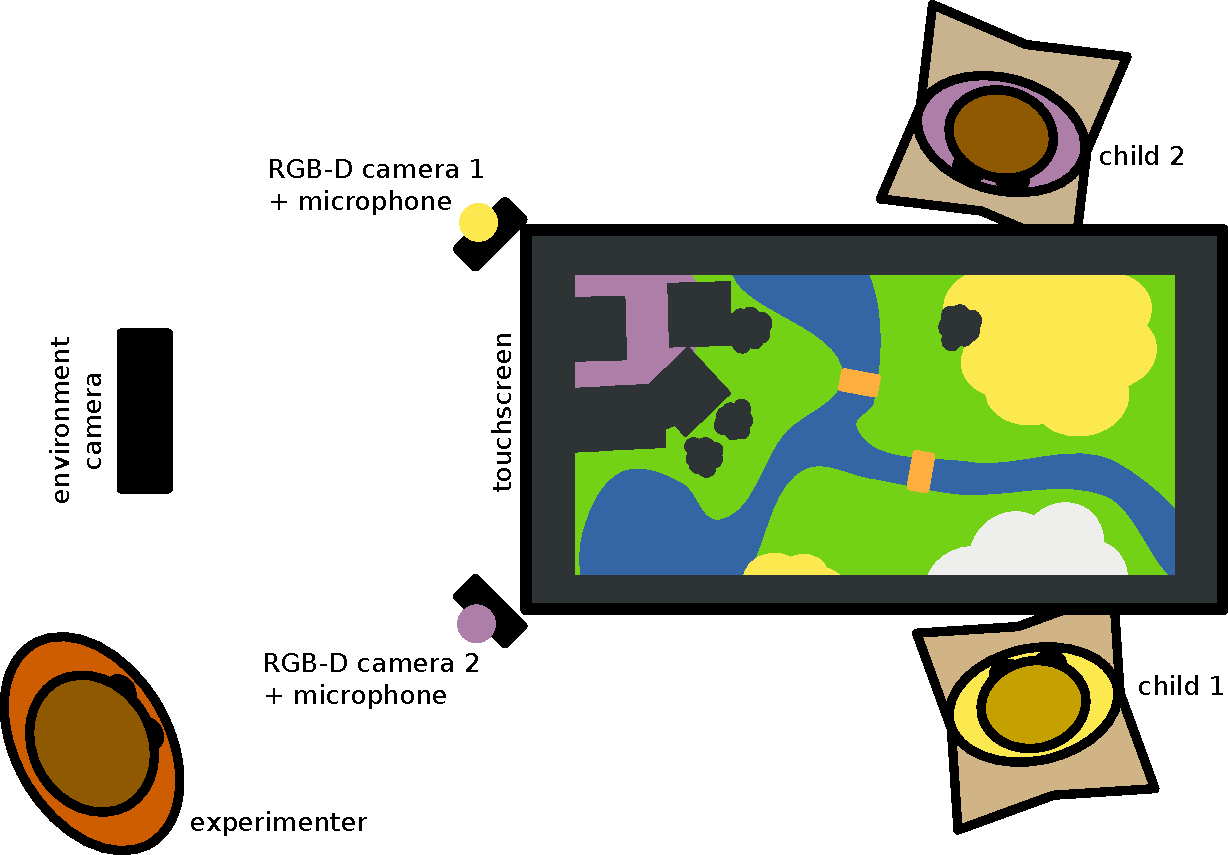
\includegraphics[width=0.4\linewidth]{setup_child_child_top}
    \hspace{1.5cm}
    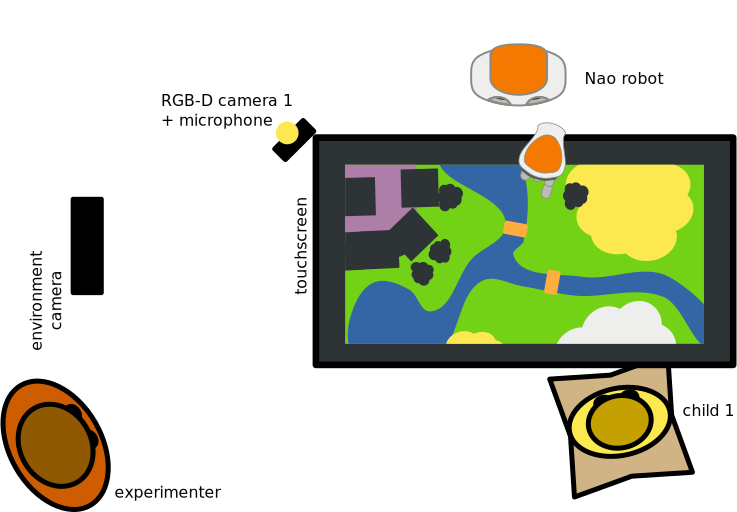
\includegraphics[width=0.4\linewidth]{setup_child_robot_top}
    \caption{Experimental setup, child-child condition (left) and child-robot
    condition (right).}
\end{figure}

The experimenter stays in the room, visible from the child. When
requested by the nursery or school, another childminder (nursery/school
staff) can be present in the room. She/he is however asked not to step
in during the experiment.

The interaction is recorded by 3 cameras (on `environment' camera
filming the whole scene; two RGB-D cameras, focused on each of the
children faces).

Audio is recorded as well with 2 microphones integrated to the RGB-D
cameras.

One computer (integrated with the touchscreen) manages the game and the
synchronous recording of the cameras and microphones.

\subsubsection{Acquisition Procedure}


\begin{enumerate}
\def\labelenumi{\arabic{enumi}.}
\item
  welcome (5 min):

  \begin{itemize}
  \item
    place children on cushions
  \item
    give them the yellow/purple sport bibs
  \item
    make sure hairs are tied (to help with face tracking)
  \item
    ask names (but do not write them down)
  \item
    fill up questionaire on the tablet -- age, gender, familiarity with
    tablet
  \item
    \textbf{remind the children that they can withdraw at anytime}
  \item
    \textbf{explain the purpose of the study: showing robots how
    children play}
  \item
    in condition B, present briefly the robot -- saying it is not a very
    sociable robot, and it might play alone.
  \end{itemize}
\item
  visual focus task (30 seconds)
\item
  tutorial (1-2 min): explain how to interact with the game, ensure the
  children are confident with the manipulation/drawing
\item
  main freeplay task (up to 40 min):

  \begin{itemize}
  \item
    start the recording
  \item
    example prompt: ``I let you play now! You can build a zoo, or tell
    stories, as you want''
  \item
    let children play
  \item
    encourage children to keep playing at least 5 min
  \item
    once they wish to stop, stop recording
  \end{itemize}
\item
  debriefing (5 min):

  \begin{itemize}
  \item
    answer possible questions from the children
  \item
    give stickers
  \end{itemize}
\end{enumerate}

\todo[inline]{mention robot greetings: expectation that the robot can talk
(and likely, hear)}
\todo[inline]{mention idea box}
\todo[inline]{mention robot calibration phase (between 0 and }

Total duration: 30 minutes per group.

\subsubsection{Initial Dataset Analysis}

analysis of behavioural alignment between partners (via
metrics like the recently proposed \emph{Individual Motor
Signature}~\cite{slowinski2016dynamic})

\begin{figure}
    \centering
    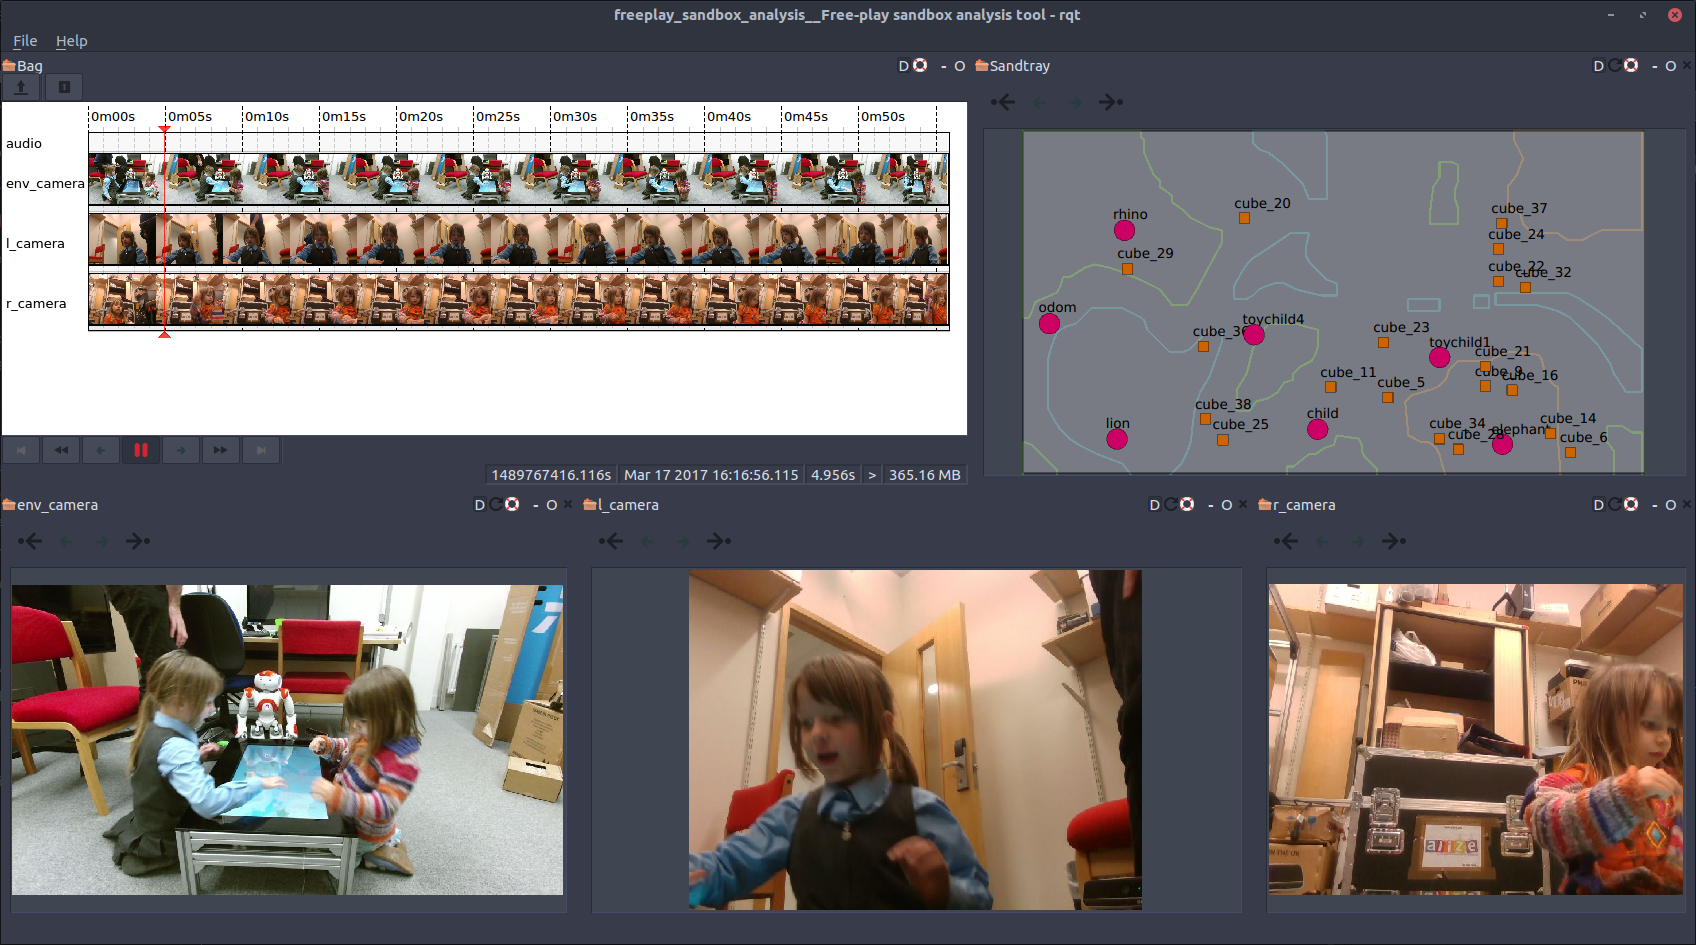
\includegraphics[width=\linewidth]{analysis}
    \caption{Screenshot of the interaction analysis tool: faces of the two
    children are recorded, as well as any interaction occuring on the
    interactive table.}
    \label{fig|analysis}
\end{figure}

\section{The PInSoRo Dataset}

\subsection{Structure}

The dataset consists in a collection of records. Each record correspond to one
play interaction between two children. To date (June 2017) 19 records have been acquired. At the end of the acquisition campaign
(July 2017), the dataset is planned to include 50 records (\ie 100 children). As
mentioned above, the duration of each play episode varies ($M=17m13s,
SD=8m02s$), but it is capped to a maximum of 40 minutes.

\todo[inline]{update with last nb before submitting}

Data is collected using the ROS middleware\footnote{\url{http://ros.org}} and
recorded as \emph{bag} files. Every dataframe is timestamped.
Table~\ref{table|datastreams} lists all the recorded datastreams.

\begin{table}[]
\centering
\caption{List of datastreams stored in each record}
\label{table|datastreams}
\begin{tabular}{@{}lll@{}}
\toprule
\bf Domain  & \bf Type                              & \bf Details                          \\ \midrule
child 1     & audio                                 & 16kHz, mono, semi-directional        \\
            & face (RGB)                            & qHD (960$\times$540), 30Hz           \\
            & face (depth)                          & VGA (640$\times$480), 30Hz           \\
            & facial features                       & 68 3D points (point cloud)           \\ \midrule
child 2     & audio                                 & 16kHz, mono, semi-directional        \\
            & face (RGB)                            & qHD (960$\times$540), 30Hz           \\
            & face (depth)                          & VGA (640$\times$480), 30Hz           \\
            & facial features                       & 68 3D points (point cloud)           \\ \midrule
environment & RGB                                   & qHD (960$\times$540), 29.7Hz         \\ \midrule
touchscreen & background drawing (RGB)              & 4Hz                                  \\
            & touches                               & 6 points multi-touch                 \\
            & items position and orientation        &                                      \\ \midrule
others      & \multicolumn{2}{l}{annotations of social behaviours and remarkable events}   \\
            & \multicolumn{2}{l}{static transforms between touchscreen and facial cameras} \\
            & \multicolumn{2}{l}{cameras calibration informations}                         \\ \bottomrule
\end{tabular}
\end{table}

As the data is recorded using ROS's bag files, it can be replayed in the exact
same conditions as it was during the recording. All the video streams use
calibrated cameras. While the raw RGB and depth streams are neither rectified
nor registered together (due to performance considerations during the
recording), it can be easily achieved as a post-process step, using standard ROS
tools (the ROS {\tt rgbd\_pipeline}). Pre-configured scripts are available
alongside the
dataset\footnote{Available online from
\url{https://github.com/severin-lemaignan/freeplay-sandbox-analysis}.} to
republish registered streams and the corresponding 3D point-clouds (as seen in
Figure~\ref{fig|pointcloud}).

\subsection{Dataset availability}
\label{availability}


The dataset is freely available to any interested researcher. Due to ethical
and data protection regulations, the dataset is however made available in two
forms: a public, Creative-Commons licensed, version that do not include any
material enabling the identification of the children (in particular, it does not
contain any video stream); and a complete version that includes all video
streams. This second version is freely available as well, but interested
researchers must first fill a data protection form.


\section{Discussion}

\subsection{Specific research questions}

\begin{figure}
\centering

\resizebox{0.8\linewidth}{!}{%
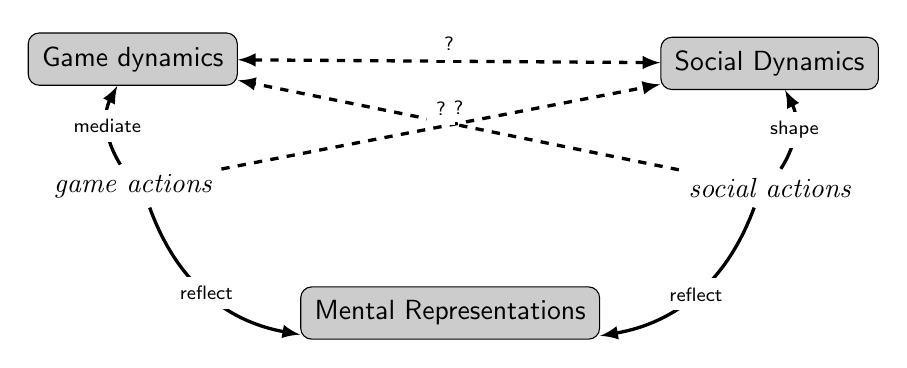
\begin{tikzpicture}[
                font=\sffamily,
                >=latex,
                every edge/.style={draw, very thick},
                node/.style={draw, rounded corners, align=center, inner sep=5pt, fill=black!20},
                label/.style={midway, align=center, font=\scriptsize\sffamily, fill=white}]

    %%% NODES
    \node [node] (mentalrepresentations) {Mental Representations};
    \node [above left=of mentalrepresentations] (gameactions) {\it game actions};
    \node [node, above=of gameactions] (gamedynamics) {Game dynamics};
    \node [above right=of mentalrepresentations] (socialactions) {\it social actions};
    \node [node, above=of socialactions ] (socialdynamics) {Social Dynamics};

    %%% CONNECTIONS
    \path (gamedynamics) edge [<->, dashed] node[label, above] {?}(socialdynamics);
    \path (gamedynamics) edge [<-, bend right] node[label] {mediate}(gameactions);
    \path (socialactions) edge [->, bend left] node[label] {reflect}(mentalrepresentations);
    \path (socialactions) edge [->, dashed] node[label,above] {?}(gamedynamics);
    \path (gameactions) edge [->, dashed] node[label,above] {?}(socialdynamics);
    \path (gameactions) edge [->, bend right] node[label] {reflect}(mentalrepresentations);
    \path (socialdynamics) edge [<-, bend left] node[label] {shape}(socialactions);

\end{tikzpicture}
}
\label{fig|researchquestions}
\caption{Game dynamics, social dynamics and mental representations are linked
    with each other through social actions (implicit and explicit communication)
    and actions on the environment (mainly game actions)}
\end{figure}

The mechanisms underlying the social interactions happening during free play
raise important questions for social robotics.


\subsubsection{Game Dynamics}

\begin{itemize}
    \item do we observe a sequence of sub-games?
    \item how are these sub-games initiated?
    \item how does A keep track of what B is playing at?
    \item how do we segment the action flow into meaningful play situations?
\end{itemize}

\subsubsection{Social Dynamics}

\begin{itemize}
    \item does a ``social protocol'' establish?
    \item if so, what are these social rules?
    \item implicit vs explicit rule setting?
    \item what interaction modalities (or combination thereof) are relied upon
        to establish and maintain this ``social protocol''?
\end{itemize}

\subsubsection{Mental representations}

\begin{itemize}
    \item Does A know what B is thinking of at time t?
    \item Do the participants perform explicit grounding of their respective mental models
        (ie, ask the other one what she is doing/thinking/planning to do?)
    \item How does the implicit grounding take place? attention tracking?
    \item Do we need at all to know what the other intends to do to actually
        collaborate? surface alignment vs deep grounding
    \item Procedural (how do you do it?) vs Semantic
        grounding (what are you doing? playing at?)
\end{itemize}

\subsection{Child-robot baseline}

During the acquisition campaign for the PInSoRo dataset, we have also recorded a
\emph{child-robot} interaction baseline. We were using the exact same protocol
as described above, only with one child replaced by a Nao robot.

The robot was fully autonomous, and programmed to exhibit a non-social behaviour
(its action policy was simply to repeatedly move interactive items to
pre-defined zones, entirely ignoring its child partner).

As such, this behaviour (and the resulting reaction of the children to a
robot acting in a non-social way) represent an experimental baseline against which
future work can be compared.


\subsection{Analysis of the free play sandbox}

Our free play sandbox elicits a loosely structured play situation. The
situation is indeed essentially aimless (free play). The goals and play episodes
that we observe during the interactions are not pre-defined, and essentially
unknown until they are decided by the players. In this sense, the free play
sandbox permits and elicits what is fundamentally \emph{unstructured play}.

However, a second look reveals some important structuring elements.

First, the physical bounds of the sandbox (an interactive table) limit the
play zone to a well defined and relatively small area. As a consequence,
children are mostly static (they are sitting in front of the table) and their
primary form of interaction is 2D pick and place of items by drag and dropping
them on the screen.

Second, the game items themselves structure the game scenarios. Items are either
iconic characters (animals or children) or plain blocks
(Figure~\ref{fig|sandbox}). The former have strong semantics associated to them
(like 'crocodiles like water and eat children'), while the later have little
semantics associated. The game background, with its recognizable zones, also
elicit a particular type of games (like building a zoo or pretending we explore
the savannah).

Finally, the social setting (two players facing each other) implicitely invites
social interaction: onlooker play, for instance, is unlikely to be observed as
the children are physically engaged with the game and the other participant
(they are sitting in front of game, close to each other). The three higher forms
of social play listed by Parten (parallel play, associative play and cooperative
play) are however possible with this setup.


Two more elements (the role and place of the experimenter, and the initial
prompt given to the participant) have an important impact on the shape of the
play situation. We discuss separately these two points in the description of the
experimental procedure.

Overall, the free play sandbox supports a \emph{loosely structured} form of play: the
actual play situations are not known and might change several times during the
interaction; the game actions, even though all based on a single modality (picking and
placing game items), are unlimited; the social interactions between participants
are multi-modal (speech, body postures, gestures, facial expressions, etc.) and
unconstrainted. However, the broad domain of the play situations and the range of
possible social interactions is bound by the physical bounds of the play zone
and the theme of the game items.

\subsection{Forms of play elicited by the sandbox}

\begin{itemize}
    \item dramatic play
    \item storytelling
    \item creative play
    \item pretend play
\end{itemize}

\section{Conclusion}


By analyzing them from the
perspective of artifical socio-cognition and human-robot interaction, we
evidence key social patterns and show that robots can recognise them,
interpret them, and (where applicable) generate them in a task-agnostic
fashion. By subsequently reusing these social patterns in similar
child-robot free play situations, we show a significant increase of the
interaction duration.



\bibliography{biblio}

\end{document}
